\documentclass[times, utf8, diplomski, numeric]{fer}
\usepackage{booktabs}
\usepackage{tabu, multirow}
\usepackage{tabularx}
\usepackage{float}
\usepackage{pdfpages}
% \usepackage{hyperref}
\usepackage{listings}
\usepackage{tikz}
\usetikzlibrary{trees}

\begin{document}

\tikzstyle{every node}=[anchor=west]
\lstset{language=c, xleftmargin=.1\textwidth, xrightmargin=.1\textwidth}

\renewcommand{\labelitemi}{$\bullet$}
\renewcommand{\labelitemii}{$-$}

% TODO: Navedite broj rada.
\thesisnumber{1995}

% TODO: Navedite naslov rada.
\title{Proširenje LTZVisor monitora virtualnih strojeva \\za višejezgrene procesore}

% TODO: Navedite vaše ime i prezime.
\author{Magdalena Halusek}

\maketitle

% Ispis stranice s napomenom o umetanju izvornika rada. Uklonite naredbu \izvornik ako želite izbaciti tu stranicu.
% \izvornik
\includepdf[pages=-,pagecommand={}]{0688_001.pdf}

% Dodavanje zahvale ili prazne stranice. Ako ne želite dodati zahvalu, naredbu ostavite radi prazne stranice.
\zahvala{}

\tableofcontents

\chapter{Uvod}
Neke od važnih odrednica ugradbenih računala su pouzdanost, predvidljivost i rad u stvarnom vremenu.
Povećanjem popularnosti IoT (engl. \textit{Internet of Things}) uređaja u industriji, počinje se isticati
još jedna dodatna karakteristika, a radi se o sigurnosti uređaja. Kako bi se uređaji u industriji osigurali,
ARM već dugi niz godina daje podršku Cortex-A procesorima \textit{TrustZone} sigurnosnim ekstenzijama.
Izlaskom M profila nove ARMv8 arhitekture, pojavila se i posebno razvijena \textit{TrustZone-M} sigurnosna
podrška Cortex-M procesora. Iako je \textit{TrustZone-M} sigurnosna ekstenzija razvijena ispočetka konkretno
za mikrokontrolere, krajnja funkcionalnost je slična onoj koju pruža \textit{TrustZone} ekstenzija Cortex-A
procesora.\\
U ovom radu će biti opisana \textit{TrustZone} sigurnosna ekstenzija ZedBoard platforme koja implementira
Cortex-A9 procesor s dvije jezgre te sustav za procesiranje (engl. \textit{Processing System}, PS) i programabilnu
logiku (PL). Kao primjer maksimalnog iskorištenja \textit{TrustZone} sigurnosne
ekstenzije, bit će prikazan LTZVisor monitor virtualnih strojeva (engl. \textit{hypervisor} ili engl.
\textit{Virtual Machine Monitor}). LTZVisor omogućava virtualizaciju u ugradbenim računalima, odnosno konkurentno
izvođenje dva operacijska sustava na jednoj jezgri procesora. Pojavom IoT uređaja u industriji, pojavila
se i sve veća potreba za virtualizacijom zbog potrebe za karakteristikama operacijskih sustava za rad u stvarnom
vremenu i operacijskih sustava opće namjene. Specifičnije, karakteristike operacijskog sustava za rad u
stvarnom vremenu koje su potrebne su odziv u stvarnom vremenu, determinizam i pouzdanost. Operacijski
sustav opće namjene je često tražen zbog dobre mrežne podrške koju nudi. U nastavku će biti opisano kako
\textit{TrustZone} doprinosi izolaciji između navedenih operacijskih sustava. Pošto je LTZVisor monitor
virtualnih strojeva namijenjen jednoj jezgri procesora, u ovom radu će se opisati postupak prilagođenja
LTZVisora za obje jezgre ZedBoarda kako bi se maksimalno iskoristile mogućnosti platforme.

\chapter{Arhitektura Cortex-A9 procesora}
APU (engl. \textit{Application Processing Unit}) Zynq-7000 platforme može sadržavati jednu ili dvije jezgre, odnosno jedan
ili dva Cortex-A9 procesora \cite{zynq_trm}. ZedBoard sadrži dva Cortex-A9 procesora \textit{little-endian} arhitekture s
koprocesorskom podrškom u višejezgrenoj konfiguraciji. Dva CPU-a dijele \textit{cache} memoriju druge razine,
odnosno L2 \textit{cache} memoriju, od 512~kB.
Oba procesora su visokih performansi i niske potrošnje. Za razliku od L2 \textit{cache} memorije, L1 \textit{cache}
memorija nije dijeljena između procesora te svaki procesor implementira odvojenu podatkovnu i instrukcijsku
L1 \textit{cache} memoriju od 32~kB. Platforma ima potpunu podršku sustava virtualne memorije ARMv7 arhitekture kojoj
pripadaju procesori ZedBoard platforme. Procesori podržavaju 32-bitne ARM i Thumb instrukcijske setove te 16-bitne
Thumb instrukcije i 8-bitne Java bajt kodove. Prisutna je i SCU (engl. \textit{Snoop Control Unit}) koja je nužna za održavanje
koherencije za L1 \textit{cache} memoriju između dva procesora. Komunikacija između PL-a i APU je ostvarena
pomoću ACP (engl. \textit{Accelerator Coherency Port}). Ispitivanje i kontrola procesora se odvija pomoću DAP-a
(engl. \textit{Debug Access Port}). Procesori podržavaju različite načine radova, uključujući \textit{supervisor},
sustavski (engl. \textit{system}) i korisnički (engl. \textit{user}) način rada što omogućava različite razine
zaštite na aplikacijskoj razini. \textit{TrustZone} ekstenzija procesora omogućava razvoj sigurnog okruženja za
izvođenje aplikacija i čuvanje njihovog sadržaja. Kako bi se minimizirao utjecaj strojnih ciklusa koji su potrebni
za izvođenje instrukcija grananja, Cortex-A9 implementira statičko i dinamičko predviđanje grananja (engl.
\textit{branch prediction}). Statičko predviđanje je određeno za vrijeme prevođenja koda, a dinamičko koristi
ishod izvođenja prošle instrukcije kako bi se odredilo hoće li se predviđeno grananje izvesti ili ne. Neka od
grananja koja se mogu predvidjeti su uvjetna i bezuvjetna grananja te se navedeno dinamičko grananje može isključiti.
Platforma sadrži i MMU (engl. \textit{Memory Management Unit}) jedinicu koja je prilagođena višeprocesorskim i sigurnosnim
ekstenzijama.

\section{Pokretanje i konfiguracija sustava}
Nakon postavljanja izvornih vrijednosti koje se odvija nakon dovođenja napajanja (engl. \textit{power
on reset}), hardver ispituje izvode platforme koji sadrže informaciju o tome na koji način će se pokrenuti sustav na
platformi. Moguće pokretanje sustava je s SD kartice, preko JTAG (engl. \textit{Joint Test Action Group}) modula
ili QSPI (engl. \textit{Quad Serial Peripheral Interface}) memorije. Nakon inicijalnog
čitanja izvoda, vrijednost se sprema u odgovarajući registar iz kojeg se čita na koji način se pokreće sustav sve do
nestanka napajanja platforme. Određivanjem načina pokretanja sustava započinje sam proces pokretanja, odnosno
počinje se izvoditi BootROM kod kojeg nije moguće mijenjati. Sveukupno pokretanje sustava se odvija u tri razine
koje su opisane tablicom~\ref{boot_stages}.

\begin{table}[H]
  \centering
  \caption{Razine pokretanja sustava Zynq-7000 platforme}
  \label{boot_stages}
  \begin{tabular}{|| p{2cm} | p{12cm} ||}
    \hline
    \textbf{Razina} & \textbf{Opis razine} \\
    \hline\hline
    Razina 0 & Odvija se odmah nakon postavljanja inicijalnih vrijednosti nakon dovedenog napajanja platformi.
    Radi se o BootROM kodu koji se izvodi na primarnom procesoru CPU0. BootROM kod izvodi traženje valjanog
    BootROM zaglavlja koji se nalazi u \textit{flash} memoriji uređaja s kojeg se pokreće sustav. Iz navedenog
    zaglavlja se određuje daljnji tok pokretanja sustava i prijelaz u Razinu 1. Nakon pokretanja hardvera, oba
    procesora izvode isti BootROM kod koji se nalazi na adresi 0x00000000 i služi za određivanje vlastitog
    CPU identiteta. Daljnje izvođenje BootROM koda se izvodi na primarnom, CPU0, procesoru, dok se sekundarni, CPU1,
    stavlja u WFE (engl. \textit{Wait For Event}) stanje.\\
    \hline
    Razina 1 & Odnosi se na prvostupanjski pokretač sustava ili FSBL (engl. \textit{First Stage Bootloader}) koji
    je zadužen za inicijaliziranje PS konfiguracije~\cite{zynq_swdg}. Uz inicijaliziranje, zadužen je i za konfiguriranje PL-a
    platforme s \textit{bitstream} datotekom (ako postoji). Sljedeći korak ove razine je učitavanje SSBL-a (engl.
    \textit{Second Stage Bootloader}) ili korisničke aplikacije, nakon čega slijedi i predavanje kontrole SSBL-u
    ili aplikaciji.\\
    \hline
    Razina 2 & Izvođenje korisničke aplikacije ili \textit{u-Boot} programa koji je sličan Linuxovoj ljusci te može
    poslužiti za učitavanje i pokretanje korisničke aplikacije.\\
    \hline
  \end{tabular}
\end{table}
Korisnička aplikacija mora sadržavati postupak CPU inicijalizacije, koji je sljedeći:
\begin{enumerate}
  \item{Upisati adresu tablice prekidnih vektora u odgovarajući registar}
  \item{Onesposobiti L1 \textit{cache} memoriju, TLB (\textit{translation look-aside buffers}) i predviđanje grananja}
  \item{Onesposobiti L2 \textit{cache} memoriju}
  \item{Pripremiti tablice stranica i učitati ih u fizičku memoriju}
  \item{Postaviti stog}
  \item{Učitati adresu tablice stranica u registar tablica za prevođenje}
  \item{Postaviti MMU bit u kontrolnom registru sustava}
  \item{Inicijalizirati i omogućiti L2 \textit{cahce} memoriju}
  \item{Omogućiti L1 \textit{cache} memoriju u kontrolnom registru sustava}
  \item{Skočiti na početak korisničke aplikacije}
\end{enumerate}

\subsection{Sigurno pokretanje sustava}
Sigurno pokretanje sustava se odnosi na sposobnost uređaja da provede pokretanje sustava koje učitava autentičnu i
kriptiranu PS sliku sustava i PL \textit{bitstream}. BootROM jedini može inicirati sigurno pokretanje sustava.
Ako je RSA-PSS (\textit{Rivest, Sharim and Adleman~-~Probabilistic Signature Scheme}) autentifikacija  omogućena,
BootROM će koristiti javni ključ PuK (\textit{Public Key}) za autentifikaciju FSBL-a. Omogućavanje sigurnog
pokretanja sustava se može izvesti modificiranjem BootROM zaglavlja u kojem se mora postaviti identifikator sigurnog
pokretanja sustava. Ako je sigurno pokretanje sustava omogućeno, BootROM automatski omogućuje AES (\textit{Advanced
Encryption Standard}) i HMAC (\textit{Key-hash message authentication code}) jedinice u PL-u. Kriptiranog FSBL-a, BootROM
šalje u AES i HMAC te se dekriptirani FSBL vraća u PS i kopira u \textit{on-chip} RAM (OCM). Nakon toga, PS može sigurno
dizajnirati PL slanjem kriptiranog PL \textit{bitstreama} u AES/HMAC jedinice nakon čega se dekriptirani
\textit{bitstream} primjenjuje na PL.
Prilikom pokretanja sustava s SD kartice, ako autentifikacija FSBL-a~ne prođe, uređaj ide u sigurnosno zaključavanje
ili u stanje greške. Kako je sigurno pokretanje sustava izvedeno u PL-u, BootROM mora pričekati da se PL-u dovede napajanje
prija slanja FSBL-a u PL. Nakon što se FSBL uspješno autentificira, FSBL kreće s izvođenjem. Ako je FSBL kriptiran,
preporučuje se da se i ostali podaci kriptiraju. Slike za pokretanje sustava se kriptiraju pomoću Bootgen alata kojeg nudi
Xilinxov SDK (engl. \textit{Software Development Kit}) koji traži upis ključa kriptiranja i autentični potpis (HMAC ključ i
potpis).
\section{Prekidni sustav}
Svaki CPU platforme ima set privatnih periferijskih prekida, PPI (engl. \textit{private peripheral interrupts}),
za koje svaki procesor ima mogućnost privatnog pristupa registrima. Oba procesora platforme imaju svoju kopiju privatnih
registara.
Takvoj vrsti prekida pripadaju globalno brojilo, privatno \textit{watchdog} brojilo, privatno brojilo i FIQ (engl.
\textit{Fast Interrupt Request}) i IRQ (engl. \textit{Interrupt Request}) koji dolaze s programabilne logike.
Kao i PPI, procesori također imaju mogućnost generiranja softverski generiranih prekida, SGI (engl. \textit{Software
Generated Interrupt}), s vlastitim kopijama registara za podešavanje SGI prekida. U sustavu postoje i periferijski prekidi
koji su dijeljeni između procesora~-~SPI (engl. \textit{Shared Peripheral Interrupt}) koji, ovisno o konfiguraciji,
mogu biti dostupni jednom ili oba procesora. Glavni upravitelj prekidima u sustavu je GIC (engl. \textit{Generic
Interrupt Controller}) koji prekide prosljeđuje odabranom CPU-u. Svi prekidi imaju svoj konfigurabilni prioritet
i listu CPU-a koji mogu obraditi prekid.

\subsection{GIC (engl. \textit{Generic Interrupt Controller})}
GIC je resurs platforme koji služi za konfiguriranje i upravljanje prekidima u sustavu s jednim ili više procesora
\cite{gic}.
Uključuje registre za upravljanje izvorima prekida, ponašanje prekida i povezivanje prekida s jednim ili više
procesora. Uz implementaciju sigurnosnih ekstenzija GIC-a, uvodi se funkcionalnost grupiranja prekida koja omogućuje:
\begin{itemize}
  \item{konfiguriranje svakog prekida kao Grupa~0 ili Grupa~1}
  \item{signaliziranje prekida Grupe~0 ciljanom procesoru pomoću IRQ ili FIQ}
  \item{signaliziranje prekida Grupe~1 ciljanom procesoru samo pomoću IRQ}
  \item{jedinstvenu obradu prioriteta prekida Grupe~0 i Grupe~1}
  \item{izborno zaključavanje konfiguriranja nekih prekida Grupe~0}
\end{itemize}
Kod višeprocesorskih sustava, GIC implementira dva modela obrade prekida u slučaju da je prekid namijenjen više
ili svim procesorima u sustavu. Prvi model je 1-N, gdje N procesora mogu obraditi prekid, ali se GIC pobrine da samo
jedan procesor u sustavu obradi prekid. Ostali procesori u sustavu prime nepredvidljivi (engl. \textit{spurious}) prekid.
Drugi model je N-N, gdje jedan procesor obrađuje prekid, a ostalima je prikazano stanje čekanja na obradu prekida.
Kod takvog modela se koriste određeni protokoli kako bi prekid bio obrađen jednom. U sklopu GIC-a postoji više kopija
prekida u sustavu, odnosno postoji više prekida s istim prekidnim brojem, za svaki procesor u sustavu postoji jedan prekidni
broj. GIC se može podijeliti na dvije logičke cjeline:
\begin{itemize}
  \item{jedan blok distributera}
  \item{jedan ili više blokova CPU sučelja}
\end{itemize}
Obrada prekida se odvija sljedećim redosljedom:
\begin{enumerate}
  \item{GIC određuje prekide koji su omogućeni}
  \item{GIC određuje ciljani procesor ili procesore za sve prekide koji čekaju na obradu}
  \item{Distributer prosljeđuje prekid najvišeg prioriteta odgovarajućem CPU sučelju}
  \item{CPU sučelje odlučuje je li potrebno generirati zahtjev za obradu prekida procesoru i ako treba, generirati ga}
  \item{Procesor priznaje prekid, na što GIC vraća ID prekida}
  \item{Nakon obrade, procesor signalizira kraj prekida GIC-u}
\end{enumerate}

\subsubsection{Distributer}
Distributer je dio GIC-a koji prikuplja sve izvore prekida te određuje prioritet svakog prekida. Za svako CPU sučelje u
sustavu prosljeđuje prekid najvišeg prioriteta. Distributer pruža sljedeće mogućnosti:
\begin{itemize}
  \item{globalno dozvoljavanje prosljeđivanja prekida CPU sučeljima}
  \item{omogućavanje i onemogućavanje svakog prekida}
  \item{postavljanje prioriteta svakog prekida}
  \item{postavljanje liste ciljanih procesora za svaki prekid}
  \item{postavljanje osjetljivosti svakog prekida:}
  \begin{enumerate}
    \item{osjetljivost na razinu}
    \item{osjetljivost na brid}
  \end{enumerate}
  \item{konfiguriranje prekida kao Grupa~0 ili Grupa~1}
  \item{prosljeđivanje SGI-a jednom ili više procesora}
\end{itemize}
Vidljivost stanja svakog prekida (neaktivan, aktivan, čeka na obradu) je omogućena čitanjem odgovarajućih registara.
Distributer sadrži i registre za postavljanje i brisanje stanja za čekanje na obradu perifernih prekida. Prekidi koji
su duplicirani za svaki procesor se odnose na prekide s prekidnim brojevima od 0 do 31, od kojih su od 0 do 15 SGI, a
od 16 do 31 PPI. Takvi prekidi se identificiraju pomoću prekidnog broja i procesora kojem su namijenjeni. Dupliciranje
prekida znači da distributer može istovremeno upravljati s više izvora prekida bez konflikta resursa.

\subsubsection{CPU sučelje}
CPU sučelje predstavlja sučelje za procesor koji je povezan s GIC-om. Njegova funkcija je prosljeđivanje prekida najvišeg
prioriteta procesoru, uz obzir na maskirane prekide i postavke istiskivanja prekida. CPU sučelje sadrži registar koji
služi za signaliziranje prihvaćanja prekida. Prihvaćanje prekida se izvodi čitanjem iz IAR-a (engl. \textit{Interrupt
Acknowledge Register}). Mogućnosti CPU sučelja su sljedeće:
\begin{itemize}
  \item{omogućavanje signaliziranja prekida procesoru}
  \item{potvrde prekida}
  \item{označavanje kraja obrade prekida}
  \item{postavljanje maskiranja prekidnog prioriteta}
  \item{definiranje postupka istiskivanja za procesor}
  \item{određivanje najvišeg prioriteta prekida koji čeka na obradu}
\end{itemize}

\section{Koprocesorska podrška}
ARM implementira koprocesorsku podršku koja proširuje funkcionalnosti ARM procesora. Sveukupno je implementirano 16 koprocesora:
CP0~-~CP15 \cite{arch_man}. Posebne namjene koprocesora su:
\begin{itemize}
  \item{CP15: ima funkcionalnost kontrole nad sustavom, služi za identifikaciju arhitekture i mogućnosti platforme. Drži
  kontrolu, status informacija i konfiguraciju sustava}
  \item{CP14: sadrži sustav za ispitivanje, kontrolu nad Thumb okruženjem izvođenja koda i konfiguraciju izvršavanja Java
  bajt kodova}
  \item{CP10 i CP11: zajedno podržavaju \textit{floating-point} operacije i operacije s vektorima}
  \item{CP8, CP9, CP12 i CP13: rezervirani}
  \item{CP0~-~CP7: sadrže informacije specifične za proizvođače}
\end{itemize}
Svi registri su duljine 32 bita. Pristup koprocesorskim registrima se izvodi pomoću MCR i MRC instrukcija, gdje je MCR
instrukcija za pisanje u koprocesorski registar, a MRC instrukcija za čitanje iz koprocesorskog registra.
Prilikom pristupa koprocesorskim registrima, potrebno je specificirati:
\begin{itemize}
  \item{identifikator koprocesora}
  \item{dva koprocesorska registra CRn i CRm, gdje je CRn primarni registar}
  \item{dva koprocesorska operacijska koda}
  \item{ARM-ov registar opće namjene čiji će se sadržaj kopirati u koprocesorski registar ili u koji će biti pohranjen
  sadržaj koprocesorskog registra}
\end{itemize}
Neki od vrlo važnih koprocesorskih registara koprocesora CP15 su: SCTLR (engl. \textit{System Control Register}), ACTLR
(engl. \textit{Auxiliary Control Register}), SACR (engl. \textit{Secure Access Control Register}), NSACR (engl. \textit{Non-
Secure Access Control Register}) i CPACR (engl. \textit{Coprocessor Access Control Register}). Programiranje SCTLR i ACTLR
registara je neizbježno te su njihove namjene opisane u nastavku. SCTLR registar je zadužen za globalno
omogućavanje/onemogućavanje instrukcijskog i podatkovnog \textit{cachea}, MMU jedinice i predviđanja grananja. Uz to, sadrži
i mogućnost podešavanja određenih karakteristika tablica prekidnih vektora, FIQ prekida, \textit{cache} memorije i MMU jedinice.
ACTLR registar je većinom zadužen za konfiguriranje \textit{cache} memorije. Ostali navedeni registri su detaljnije opisani u
kasnijim poglavljima.

\section{MMU (engl. \textit{Memory Management Unit})}
MMU jedinica pruža zaštitu memorije i adresna prevođenja. Stranice za tablice za prevođenje mogu imati veličine od 4~kB,
64~kB, 1~MB i 16~MB i 16 pristupnih domena (skup memorijskih regija). MMU ZedBoard platforme je prilagođena sigurnosnim
ekstenzijama i višeprocesorskim konfiguracijama. Kontrolira setove adresnih mapa za prevođenje virtualne memorije u fizičku.
Atributi memorije sadržani su u instrukcijskim i podatkovnim spremnicima za prevođenje TLB (\textit{translation look-aside
buffers}). Glavna funkcija MMU jedinice je adresno prevođenje koje služi za prevođenje adresa koda i podataka iz virtualnih u
fizičke. Omogućava dodjelu memorije zadacima na način da zadaci nemaju znanja o postojanju drugih zadataka u sustavu. Takvo
memorijsko konfiguriranje omogućuje jednostavniju implementaciju aplikacija obzirom da sve aplikacije/zadaci koriste jednak
virtualni memorijski prostor. MMU sadrži dvije glavne komponente ključne za ostvarenje adresnih prevođenja:
\begin{itemize}
  \item{pretraživač tablica koji automatski dohvaća točan ulaz tablice za prevođenje za zahtjevano prevođenje}
  \item{spremnici za prevođenje koji pohranjuju nedavno korištene ulaze za prevođenje i ponašaju se slično kao \textit{cache}
  memorija za tablice za prevođenje}
\end{itemize}
Svaka virtualna adresa odgovara točno jednom ulazu u tablicu za prevođenje. Tablice za prevođenje, uz ulaze virtualne memorije,
sadrže i dozvole pristupa i atribute memorije za odgovarajuće stranice.

\chapter{Višejezgrene konfiguracije Zynq-7000 platforme}
Kao što je već rečeno, ZedBoard implementira Cortex-A9 procesor s dvije jezgre te je za navedenu
platformu moguće razviti aplikacije s različitim konfiguracijama obzirom na broj jezgri koje su potrebne
u sustavu. Moguće je implementirati:
\begin{itemize}
  \item{aplikaciju namijenjenu jednoj jezgri (CPU0),}
  \item{dvije aplikacije, svaka namijenjena jednoj jezgri i}
  \item{aplikaciju namijenjena objema jezgrama u sustavu.}
\end{itemize}
Korištenjem prednosti višejezgrenih konfiguracija, dobiju se bolje performanse platforme u smislu da je višejezgrena platforma
sposobna obavljati N zadataka u nekom vremenskom trenutku, gde je N broj jezgri platforme \cite{cortexa_pg}. Zbog paralelnosti
obavljanja zadataka, određeni posao se može obaviti brže nego na platformi s jednom jezgrom. Nakon što obave potrebni posao,
jezgre mogu ići u stanje gašenja kako bi se smanjila potrošnja. Još jedan način smanjenja potrošnje je da se smanji frekvencija
na kojoj rade jezgre. Uz to, višejezgrene platforme mogu imati bolji odziv u odnosu na platforme s jednom jezgrom jer bilo koja
jezgra može obraditi prekid, što smanjuje broj prekida koje je potrebno obraditi na jednoj jezgri.\\
Važno je napomenuti da je jedna jezgra sustava (CPU0) primarna, a druga (CPU1) sekundarna. Prilikom
pokretanja sustava, na platformi je aktivna samo primarna jezgra, dok se sekundarna jezgra nalazi u
WFE (engl. \textit{Wait For Event}) stanju. Nakon što se sustav pokrenuo, primarna jezgra je zadužena
za buđenje sekundarne jezgre. Sekundarnu jezgru je moguće probuditi generiranjem događaja sustava
(engl. \textit{system event}), nakon čega sekundarna jezgra automatski skače na adresu koja je upisana
na lokaciji 0xFFFFFFF0. Jedan od načina na koji se može probuditi sekundarna jezgra je da aplikacija
koja se izvršava na CPU0 upiše adresu na kojoj se nalazi aplikacija za CPU1 na memorijsku lokaciju
0xFFFFFFF0 te izvrši SEV (engl. \textit{send event}) instrukciju koja rezultira buđenjem CPU1.
Komunikaciju između dvije jezgre je moguće ostvariti pomoću prekida između procesora
(engl. \textit{inter-processor interrupt}), dijeljene memorije ili razmijene poruka. Prekidi između procesora
na ovoj platformi se implementiraju pomoću softverski generiranih prekida (SGI). Za bolje razumijevanje
višejezgrenih konfiguracija, u nastavku su dani jednostavni primjeri razvoja aplikacije za dvije različite
konfiguracije. Obje aplikacije su razvijene pomoću skupa alata arm-none-eabi i Xilinx SDK 2019 (engl.
\textit{Software Development Kit}) uz zadanu konfiguraciju hardvera (bez potrebe za generiranjem
novog dizajna hardvera). Za potrebe generiranja datoteke za pokretanje sustava korišten je već gotov FSBL projekt
kojeg nudi XSDK koji ima mogućnost učitavanja više izvornih datoteka odjednom. Datoteka za pokretanje sustava je
generirana pomoću alata Bootgen kojeg nudi XSDK.

\section{Asimetrično višejezgreno procesiranje}
Asimetrično višejezgreno procesiranje ili AMP (engl. \textit{Asymmetric Multiprocessing}) se odnosi na
konfiguraciju u kojoj svaki procesor (jezgra) izvršava svoju aplikaciju, odnosno gdje svaki procesor ima
svoju sliku operacijskog sustava. Dakle, kako bi bilo moguće razviti obje aplikacije, potrebno je koristiti
odvojene skripte za memorijsko povezivanje (\textit{linker} skripte) i skripte za pokretanje sustava. Oba
operacijska sustava dijele isti fizički memorijski prostor, odnosno ne postoji nikakva izolacija između dva
operacijska sustava. Karakteristike AMP konfiguracije su sljedeće:
\begin{itemize}
  \item{većina uređaja mora biti posvećena određenom procesoru}
  \item{upravitelj prekidima je dijeljen između procesora}
  \item{samo jedan procesor je zadužen za inicijalizaciju upravitelja prekidima}
\end{itemize}
FSBL je zadužen za učitavanje obje aplikacije u memoriju. Opisana konfiguracija je prikazana slikom \ref{amp}.

\begin{figure}[H]
  \centering
	\includegraphics[width=300pt]{AMP.png}%
	\caption{AMP konfiguracija}
	\label{amp}%
\end{figure}

\subsection{Razvoj AMP aplikacije}
Kod razvoja AMP aplikacije u XSDK, nužno je stvoriti dva projekta, jedan za procesor CPU0 i drugi za CPU1.
Prilikom stvaranja projekta potrebno je odabrati za koji procesor je aplikacija namijenjena. Kod konfiguriranja
projekta za CPU1, prevoditelju projekta je potrebno dodati poseban indikator: \textit{USE\_AMP=1} kako bi aplikacija mogla
funkcionirati na ispravan način. Postavljanjem \textit{USE\_AMP} zastavice, otklanja se mogućnost rekonfiguriranja L2 \textit{cache}
memorije i distributera GIC upravitelja što se smatra nepoželjnim rukovanjem navedenih resursa koji su zajednički procesorima
u sustavu. Primjer nepoželjnog ponašanja zbog ne postavljanja navedene zastavice je dvostruka inicijalizacija distributera
GIC-a što bi moglo rezultirati gubitkom postavki prekida koje su postavljene primarnim procesorom. Takvo ponašanje bi
prekršilo jedno svojstvo AMP aplikacija koje se odnosi na to da je samo jedan procesor zadužen za inicijalizaciju upravitelja
prekidima, u ovom slučaju GIC distributera. CPU sučelje GIC-a se normalno inicijalizira na oba procesora, bez ograničenja.
Obzirom da su za razvoj AMP aplikacije potrebna dva projekta, potrebne su i dvije skripte za memorijsko povezivanje što
znači da svaki procesor mora imati svoje upravljačke programe za uređaje (engl. \textit{device drivers}) koje treba koristiti.
Ako se za primjer uzme funkcija \textit{print}, koja se koristi za ispis preko serije korištenjem UART-a (engl. \textit{Universal
Asynchronous Receiver Transmitter}), implementirana procesorom CPU0, jasno je da CPU1 neće moći pozvati tu istu funkciju
jer funkcija nije vidljiva u memorijskom prostoru CPU1 aplikacije. Da bi CPU1 mogao koristiti istu \textit{print} funkciju,
CPU1 treba implementirati funkcionalnost te funkcije kako bi skripta za memorijsko povezivanje mogla locirati navedenu
funkciju. Iz ovog se vidi da nije praktično koristiti isti uređaj na oba procesora te se zbog toga većina uređaja dodjeljuje
određenom procesoru. Iako se UART može dijeliti između procesora, neke periferije, kao što su to brojila, se ne mogu.
Za razliku od CPU0, CPU1 mora eksplicitno omogućiti prekide u kontrolnom registru procesora CPSR (engl. \textit{Current
Program Status Register}). Prekidi za CPU0 su
automatski omogućeni FSBL-om. Podrazumijeva se da CPU0 aplikacija mora sadržavati dio koda koji služi za buđenje CPU1
čime započinje pokretanje sustava na CPU1. Isto tako, podrazumijeva se i da se adresa od koje kreće CPU1 aplikacija
ispravno podesi u skripti za memorijsko povezivanje CPU1 aplikacije. Nakon što su željene aplikacije razvijene, moguće
je kreirati datoteku za pokretanje sustava BOOT.bin. Programski tok od pokretanja sustava (Razine~1) prikazana je slikom
\ref{amp_app}.

\begin{figure}[H]
  \centering
	\includegraphics[width=300pt]{AMP_app.png}%
	\caption{AMP aplikacija}
	\label{amp_app}%
\end{figure}

\section{Simetrično višejezgreno procesiranje}
Simetrično višejezgreno procesiranje ili SMP (engl. \textit{Symmetric Multiprocessing}) se odnosi na
konfiguraciju u kojoj su oba procesora ZedBoard platforme zadužena za jedan operacijski sustav, odnosno
za jednu aplikaciju. Kod razvoja SMP aplikacije potrebna je samo jedna skripta za memorijsko povezivanje, ali
dvije skripte za pokretanje sustava. U slučaju razvoja aplikacije operacijskog sustava, u sustavu postoji
samo jedan raspoređivač zadataka koji je zadužen za raspoređivanje procesa, odnosno zadataka, na obje jezgre.
Prilikom razvoja SMP aplikacije moguće je:
\begin{itemize}
  \item{odrediti procesor koji će izvoditi određeni proces,}
  \item{obraditi prekid s bilo kojim slobodnim procesorom,}
  \item{odrediti jedan procesor koji će biti zadužen za inicijalizaciju i pokretanje drugih procesora.}
\end{itemize}
SMP ima mogućnost dinamičkog određivanja uloge svakog procesora te se svaki zadatak može izvoditi na bilo kojoj jezgri.
Opisana konfiguracija prikazana je slikom \ref{smp}.
\begin{figure}[H]
  \centering
	\includegraphics[width=300pt]{SMP.png}%
	\caption{SMP konfiguracija}
	\label{smp}%
\end{figure}

\subsection{Razvoj SMP aplikacije}
Prilikom razvoja SMP aplikacije u XSDK, potrebno je stvoriti jedan projekt koji je namijenjen primarnom procesoru, CPU0.
Pošto se sustav CPU0 procesora pokreće prvi, CPU0 je zadužen za inicijalizaciju i pokretanje sustava na CPU1. Iz navedenog
se vidi da se u projekt treba dodati skripta za pokretanje sustava na CPU1. Za te potrebe, duplicirala se je boot.S skripta
koju nudi Xilinxova biblioteka. Kako razvoj SMP aplikacije ne zahtjeva poseban projekt za CPU1, potrebno je modificirati
skriptu za pokretanje sustava na CPU1 na način da se izbaci dio s inicijalizacijom L2 \textit{cache} memorije (kod AMP
aplikacije, to je ostvareno pomoću indikatora \textit{USE\_AMP}). Također, potrebno je promijeniti aplikaciju na koju se skače
nakon inicijalizacije CPU1 procesora (postaviti skok na željenu CPU1 aplikaciju u skripti za pokretanje sustava).
Poznato je da svaki procesor ima svoju tablicu
prekidnih vektora te je iz tog razloga potrebno dodati asemblerski kod koji će sadržavati potrebnu tablicu prekidnih vektora.
Tablica prekidnih vektora mora biti sadržana u memoriji koja ima odmak 0x00 od početne adrese na kojoj se nalazi
aplikacija CPU1 procesora. Da bi se ostvario potrebni odmak, poduzeti su sljedeći koraci:
\begin{enumerate}
  \item{U skriptu za memorijsko povezivanje, dodana je adresa na kojoj će se nalaziti CPU1 aplikacija}
  \item{U skriptu za memorijsko povezivanje, dodana je nova sekcija koje će sadržavati sav CPU1 kod (ili minimalno asemblerski
  kod tablice prekidnih vektora CPU1)}
  \item{U asemblerski kod tablice prekidnih vektora CPU1, dodana je direktiva .org 0 koja osigurava da se kod smjesti na
  početak odabrane sekcije (odmak 0x00 od početka memorijskog segmenta sekcije)}
\end{enumerate}
Važno je napomenuti i da CPU1 treba imati poseban stog namijenjen CPU1 procesoru te je stog potrebno dodati u skriptu za
memorijsko povezivanje. Uz to, u skriptu za pokretanje je potrebno navesti odgovarajući stog CPU1 procesora.
Nakon navedenih promjena, projekt je spreman za implementaciju aplikacije. Pošto se radi o SMP konfiguraciji, razvija se
samo jedna aplikacija koja sadrži dva zadatka koji se konkurentno izvode (jedan na CPU0, a drugi na CPU1). Također, sve
funkcije dostupne jednom procesoru su dostupne i drugom procesoru jer dijele jedan memorijski prostor (jedna skripta za
memorijsko povezivanje). Jedna ključna stavka kod razvoja SMP aplikacije je da ako oba procesora u aplikaciji pristupaju
istom resursu, za ispravno funkcioniranje je potrebno implementirati sinkronizacijski mehanizam. Sinkronizacijski mehanizam
osigurava da jednom resursu ne pristupaju oba procesora u istom trenutku. Primjer jednostavnog sinkronizacijskog mehanizma
iskorištenog u razvoju SMP aplikacije je korištenje jedne memorijske lokacije koja služi za indikaciju je li resurs slobodan.
Kao i kod AMP aplikacije, mora se pobrinuti za to da GIC distributer bude inicijaliziran samo jednom. Isto tako je potrebno
omogućiti prekide u CPSR registru CPU1 procesora u slučaju da će se prekidi obrađivati procesorom CPU1. Nakon što CPU0
probudi CPU1, CPU1 počinje izvoditi dio koda koji je smješten na početku sekcije koja je rezervirana za CPU1 kod.
Podrazumijeva se da se na odgovarajuću memorijsku lokaciju, koja sadrži informaciju o adresi na koju skače CPU1 nakon buđenja,
upiše adresa koja je jednaka početnoj adresi CPU1 sekcije. Tok programa od pokretanja sustava (Razine~1) prikazan je slikom
\ref{smp_app}.
\begin{figure}[H]
  \centering
	\includegraphics[width=300pt]{SMP_app.png}%
	\caption{SMP aplikacija}
	\label{smp_app}%
\end{figure}

\chapter{\textit{TrustZone} sigurnosna ekstenzija Cortex-A platforma}
Potreba za sigurnošću ugradbenih računala sve više raste zbog rastuće vrijednosti podataka pohranjenih na njima kao
što su to bankovni računi ili sinkronizirane \textit{e-mail} adrese \cite{tz_wp}. Povećanjem vrijednosti podataka pohranjenih na
uređaje povećava vjerojatnost napada na uređaj. Cilj \textit{TrustZone} ekstenzije je pružiti robusno sigurnosno okruženje
uređajima bogatih operacijskih mogućnosti, integrirajući zaštitne mjere u ARM-ov procesor, sabirnički sustav i periferijski
sustav. Kako bi se odredile mjere zaštite, potrebno je odrediti napade od kojih se želi zaštititi, odnosno koji resursi
moraju biti zaštićeni.

\section{Potreba za sigurnosti u mobilnom sektoru}
Dvije kritične komponente mobilnih uređaja su IMEI (engl. \textit{International Mobile Equipment Identity}) kod i
\textit{SIMLock}. IMEI je jedinstveni kod koji se koristi za identifikaciju uređaja kad se priključi na mrežu te se prilikom
krađe uređaja koristi za zabranu pristupa mreži. \textit{SIMLock} je protokol koji se koristi za povezivanje uređaja i
SIM kartice određenog operatera te se kod krađe uređaja koristi za vezanje uređaja i operatera do isteka ugovora. Ovakvi
zaštitni mehanizmi se mogu lako premostiti (obično reprogramabilnim alatom i USB kablom). O tome koliko je jednostavno
srušiti takve sigurnosne mehanizme, govori statistika Ujedinjenog Kraljevstva koja iznosi da se pola od ukupnih uličnih
zločina odvija preko krađe mobilnih uređaja što donosi velike novčane štete industriji. Noviji uređaji imaju dodatne
zaštitne mehanizme koji se odnose na sadržaj i servise koji su dostupni lokalno na uređaju. Kritične značajke novih
uređaja su sinkronizirane \textit{e-mail} adrese, povećane mogućnosti žične i bežične povezanosti i velike količine
podatkovne memorije. Primjer industrije koja nije otvorenog sustava je automobilska industrija koja također snosi velike
novčane štete zbog napada na ugradbena računala. Sigurnosne značajke potrebne kod takvih ugradbenih sustava su autentičnost
nadogradnje ugrađenog softvera i osiguranje da se ispitivanje sustava ne može zlonamjerno iskoristiti.
Takve značajke se mogu implementirati pomoću \textit{TrustZone} ekstenzije. Prilikom dizajna sigurnosnog rješenja, proizvođač
mora izmjeriti omjer cijena koje mora uložiti u dizajn i štete koju bi mogao imati zbog napada. Zbog niže kompleksnosti
izvedbe \textit{TrustZone} ekstenzije, ARM ima i niže troškove proizvodnje ekstenzije što ide u prilog proizvođačima
uređaja.

\section{Softverska virtualizacija}
Virtualizacija je jedan od načina kako ostvariti sigurnosni mehanizam u kojem se visoko pouzdani sloj za upravljanje,
odnosno monitor virtualnih strojeva, izvodi u privilegiranom načinu rada procesora. Monitor virtualnih strojeva razdvaja
više neovisnih softverskih okruženja, koja se izvode povrh monitora, koristeći MMU. Svako softversko okruženje je
smješteno u virtualni stroj kojim upravlja monitor virtualnih strojeva. Virtualni strojevi su sigurni od međusobnih softverskih
napada virtualnih strojeva upravo zato što njima upravlja monitor virtualnih strojeva. Ovakav opis virtualizacije pripada
paravirtualizaciji koja je specifična za ugradbena računala. Za implementaciju monitora virtualnih strojeva, minimalan
hardverski uvjet je prisutnost MMU jedinice što predstavlja prednost ovako ostvarenog sigurnosnog mehanizma. Sigurnosno
osjetljive aplikacije mogu biti smještene u sigurnosno okruženje unutar monitora virtualnih strojeva. Nadalje, monitor
virtualnih strojeva omogućuje mehanizam komunikacije između virtualnih strojeva. Iako se softverska virtualizacija čini kao
čvrst oblik sigurnosnog mehanizma, ipak postoji skup sigurnosnih značajki koje ne zadovoljavaju sigurnosne uvjete. Primjer
jedne od njih je da virtualizacija osigurava izolaciju samo na razini procesora. Ako se u sustavu želi zaštititi DMA (engl.
\textit{Direct Memory Access}) jedinica, koja ostaje nezaštićena, potrebno je omogućiti mehanizam upravljanja DMA jedinicom
u softverskom sloju monitora virtualnih strojeva što znatno usporava cijeli sustav. Isto tako, virtualizacija ne nudi nikakvu
hardversku zaštitu te sustav može biti lako ranjiv kroz sustav za ispitivanje (JTAG).

\section{\textit{TrustZone} arhitektura}
Općeniti problem sigurnosnih mehanizama je da štite samo određene resurse. Kao primjer se mogu uzeti kriptografički blokovi
platforme koji se koriste za zaštitu ključeva. Takvi blokovi gube svoju glavnu funkciju ako nisu zaštićeni i dekriptirani
podaci izvan kriptografičkih blokova. Ideja \textit{TrustZone} ekstenzije je dati mogućnost zaštite cjelokupnog hardverskog
prostora. Ekstenzija pruža konfigurabilni sustav kojeg dizajner može konfigurirati na način koji je specifičan za željenu
aplikaciju. AMBA3 AXI sabirnički protokol omogućava \textit{TrustZoneov} koncept dva svijeta: Sigurnog (\textit{Secure}) i
Nesigurnog ili Normalnog (\textit{Non-Secure}) svijeta. Smještanje osjetljivih resursa u Sigurni svijet štiti uređaj i od napada
od kojih se je teško obraniti, kao što je to unošenje lozinke putem tipkovnice ili dodirnog zaslona.
Kako bi takva konfiguracija bila moguća, \textit{TrustZone} sadrži tri ključne komponente:
\begin{itemize}
  \item{TZPC (\textit{TrustZone Protection Controller}) - omogućava dinamičku izmjenu sigurnosnog stanja prilikom izvođenja
  programa}
  \item{TZASC (\textit{TrustZone Address Space Controller}) - omogućava podjelu memorije na Sigurne i Nesigurne segmente}
  \item{TZMA (\textit{TrustZone Memory Adapter}) - omogućava označavanje segmenata statičke memorije kao Sigurna memorija}
\end{itemize}
Ekstenzija samog procesora
omogućava efektivno izvođenje koda Normalnog i Sigurnog svijeta pomoću metode vremenskog dijeljenja (\textit{time-sliced
fashion}). Ključna mogućnost ekstenzije je kontroliranje pristupa ispitivanja Sigurnog softvera. Promjena uvedena u AMBA3
AXI sabirnicu je dodavanje 33. NS (\textit{Non-Secure}) bita prilikom čitanja i pisanja. Dodatni bit indicira s kojeg
svijeta dolazi zahtjev za razmjenu podataka te onemogućava pristup Nesigurnog svijeta Sigurnom. Sigurnost periferija je
izvedena pomoću AXI-APB mosta, gdje je APB (engl. \textit{Advanced Peripheral Bus}) sabirnica na koju su spojene
periferije. APB ne implementira dodatni bit kao AXI sabirnice te je stoga AXI-APB most zadužen za provjeru valjanosti
zahtjeva. Takvo svojstvo omogućuje osiguravanje tipkovnice za potrebe unosa lozinke. Ekstenzija procesora uvodi dvije virtualne
jezgre za svaki procesor, gdje je jedna virtualna jezgra zadužena za Sigurni, a druga za Nesigurni svijet kako je prikazano na
slici \ref{vcpu}. Na slici, oznaka VCPU označuje virtualni CPU.
\begin{figure}[H]
  \centering
	\includegraphics[width=200pt]{vcpu2.png}%
	\caption{Virtualizacija fizičkog procesora}
	\label{vcpu}%
\end{figure}
Uz promjenu na
sabirnici, \textit{TrustZone} uvodi i novi način rada procesora: nadgledni (\textit{monitor mode}) uz dva stanja: Sigurno
i Nesigurno stanje. Nadgledni način rada je uvijek u Sigurnom stanju.\\
Koncept dva svijeta se može gledati kao dva zadatka u operacijskom sustavu, gdje je softver koji se izvodi
u nadglednom načinu rada zadužen za zamjenu konteksta između dvije virtualne jezgre. Pokretanje cjelokupnog sustava s dva
svijeta prikazano je slikom~\ref{tz_boot}.
\begin{figure}[H]
  \centering
	\includegraphics[width=350pt]{tz_boot.png}%
	\caption{Pokretanje \textit{TrustZone} sustava}
	\label{tz_boot}%
\end{figure}
Sigurno pokretanje sustava dodaje kriptografičke provjere za svaku razinu pokretanja Sigurnog svijeta.
Prijelazi iz Nesigurnog stanja u nadgledni
način rada se izvode pomoću SMC (engl. \textit{Secure Monitor Call}) instrukcije ili konfiguracijom IRQ kao okidač za ulaz
u nadgledni način rada. Identifikacija svijeta u kojem se softver izvodi se nalazi u NS bitu SCR (\textit{Secure
Configuration Register}) registra CP15 koprocesora. Samo Sigurni softver može upravljati NS bitom SCR registra. Postavljanjem
NS bita u jedinicu se okida zamjena konteksta iz Sigurnog svijeta u Nesigurni svijet. \textit{TrustZone} predstavlja i
virtualnu MMU jedinicu, gdje je jedna virtualna MMU jedinica zadužena za jedan virtualni procesor. Opisnik tablice za prevođenje
sadrži NS polje koje dozvoljava Sigurnom softveru pristupanje Sigurnoj i Nesigurnoj tablici, a onemogućava pristup Sigurnoj
tablici od strane Nesigurnog softvera. Uz MMU, L1 \textit{cache} memorija se također dijeli na Sigurnu i Nesigurnu.\\
Softver nadglednog načina rada je zadužen za prijelaz između Sigurnog i Nesigurnog stanja te osigurava spremanje konteksta
svijeta iz kojeg prelazi i točnog povratka konteksta svijeta u koji se vraća. Za jednostavnost implementacije, preporučuje
se isključivanje prekida prilikom izvođenja nadglednog softvera. Sigurno stanje registara treba pospremiti u Sigurnu memoriju
gdje Nesigurni svijet ne može pristupiti Sigurnom kontekstu. Implementacija \textit{yield} funkcije se izvodi pomoću SMC
instrukcije koja može nositi i korisnu informaciju te u tom slučaju nadgledni način rada ne radi potpunu zamjenu konteksta.
Za smanjenje vremena zamjene konteksta, Sigurni softver može ograničiti Nesigurni pristup koprocesorskom sučelju te ako se
izabere takva konfiguracija, nadgledni način rada izvodi lijenu zamjenu konteksta.

\subsection{Utjecaj sigurnosnih ekstenzija na prekidni sustav}
GIC je svjestan sigurnosnih ekstenzija i daje mogućnost konfiguriranja Sigurnih i Nesigurnih prekida. Kod prekidnog sustava,
ARM preporučuje korištenje IRQ kao Nesigurne prekide, a FIQ kao Sigurne prekide što je konfigurabilno u GIC-ovim registrima.
Ako se koristi takav model, preporučeno je da se prilikom prijelaza u Nesigurni svijet SCR registar podesi tako da se izbriše
IRQ bit, a postavi FIQ bit. Kod prijelaza u Sigurni svijet preporučeno je podesiti SCR registar tako da se postavi IRQ bit, a
izbriše FIQ bit.
Sigurnosne ekstenzije omogućuju tri vrste tablica prekidnih vektora:
\begin{itemize}
  \item{za Sigurni svijet}
  \item{za Nesigurni svijet}
  \item{za nadgledni način rada}
\end{itemize}
Memorijsko mapiranje spomenutih tablica prekidnih vektora dano je tablicom \ref{vector_table}.
\begin{table}[H]
  \centering
  \caption{Tablice prekidnih vektora}
  \label{vector_table}
  \begin{tabular}{|| p{2cm} | p{4cm} | p{4cm} | p{4cm} ||}
    \hline
    \textbf{Memorijski odmak} & \textbf{Nesigurna tablica} & \textbf{Sigurna tablica} & \textbf{Nadgledna tablica} \\
    \hline\hline
    0x00 & Ne koristi se & \textit{Reset} & Ne koristi se\\
    \hline
    0x04 & Nedefinirana instrukcija & Nedefinirana instrukcija & Ne koristi se\\
    \hline
    0x08 & Poziv \textit{supervisoru} & Poziv \textit{supervisoru} & Sigurni poziv nadgledniku (SMC)\\
    \hline
    0x0C & \textit{Prefetch abort} & \textit{Prefetch abort} & \textit{Prefetch abort}\\
    \hline
    0x10 & \textit{Data abort} & \textit{Data abort} & \textit{Data abort}\\
    \hline
    0x14 & Ne koristi se & Ne koristi se & Ne koristi se\\
    \hline
    0x18 & IRQ & IRQ & IRQ\\
    \hline
    0x1C & FIQ & FIQ & FIQ\\
    \hline
  \end{tabular}
\end{table}
Bazna adresa Sigurne tablice prekidnih vektora može biti 0x0 ili 0xFFFF0000, dok se ostale adrese određuju softverski.
Nesigurni prekidi nemaju mogućnost konfiguriranja Sigurnih prekida te je opredjeljenje prekida kao Sigurni ili Nesigurni
moguće samo u Sigurnom softveru. Sigurni softver može osigurati da su svi Sigurni prekidi većeg prioriteta od Nesigurnih.
To je moguće jer prioritetni registar prekida u Sigurnom stanju ima implementirano 5 bitova, dok u Nesigurnom stanju ima
implementirano 4~bita.
Prekid Grupe 0 GIC-a se označava kao Sigurni prekid, a prekid Grupe 1 kao Nesigurni prekid. Pristup GIC-ovim registrima uz
sigurnosne ekstenzije imaju sljedeće značajke:
\begin{itemize}
  \item{Nesigurno čitanje polja registra koje sadrži informaciju o Sigurnom prekidu vraća 0}
  \item{GIC ignorira svako Nesigurno pisanje u polje registra koje drži informaciju o Sigurnom prekidu}
  \item{Sigurni softver posebno određuje koji prekidi će se koristiti kao Sigurni, a koji kao Nesigurni}
  \item{Nesigurni prekid signalizira IRQ zahtjev ciljanom procesoru}
  \item{Sigurni softver signalizira IRQ ili FIQ zahtjev ciljanom CPU-u}
  \item{Sigurni softver može upravljati prekidnim izvorima bez interferencije Nesigurnog softvera}
  \item{Sigurni softver se može koristiti i kao softver koji nije svjestan sigurnosnih ekstenzija}
\end{itemize}
ARM preporučuje korištenje prekida kao komunikaciju između procesora u sljedećoj konfiguraciji:
\begin{itemize}
  \item{Nesigurni prekidi: prekidi s prekidnim brojevima od 0-7}
  \item{Sigurni prekidi: prekidi s prekidnim brojevima od 8-15}
\end{itemize}

\subsection{Višejezgrene konfiguracije \textit{TrustZone} ekstenzije}
Jedan fizički procesor i njegova dva virtualna procesora čine jednu grupu procesora. Svaka grupa može biti konfigurirana za
korištenje u AMP ili SMP modelu. Kod SMP modela, korištenje L1 \textit{cache} memorije na oba procesora je koherentno što
je omogućeno SCU jedinicom. Prilikom razvoja AMP aplikacije, mora se ručno voditi briga o koherenciji (prazniti \textit{cache}
gdje je potrebno). Prijelaz između svjetova na jednom procesoru je neovisan o drugim procesorima. Za povećanje sigurnosti
prilikom implementacije Sigurnog softvera u višeprocesorskim sustavima, preporučuje se da Sigurni softver ne iskorištava
mogućnosti više procesora, iako Nesigurni softver možda i iskorištava. Razlog tome je kompleksnost implementacije što povlači
veću vjerojatnost pogreške, odnosno sustav postaje ranjiviji. Ako Sigurni softver ne koristi višeprocesorske mogućnosti,
a Nesigurni koristi potrebno je implementirati sinkronizaciju komunikacije između SMP Nesigurnog softvera i Sigurnog softvera.
Obzirom na SMP, moguće je ostvariti dva modela:
\begin{enumerate}
  \item{Sigurni softver implementiran na jednom procesoru, a Nesigurni na oba (konfiguracija s 4 procesora u sustavu prikazana
  je na slici \ref{smp_tz})}
  \item{Sigurni softver mijenja procesor na kojem je aktivan, a Nesigurni koristi oba procesora}
\end{enumerate}
Prednost prvog modela je jednostavnost prosljeđivanja prekida Sigurnom softveru, a nedostatak što raspoređivač zadataka
Nesigurnog softvera postaje neefikasan zbog dodjeljivanja procesorskog vremena Sigurnom softveru. Prednost drugog modela je
što rješava problem s raspoređivačom zadataka Nesigurnog softvera, ali prosljeđivanje prekida Sigurnom softveru postaje
kompleksno. Softver nadglednog načina rada se mora pobrinuti da Nesigurni softver procesora kojeg ne koristi i Sigurni softver
ne zatraži zahtjev za zamjenu konteksta. Kad bi zahtjevi bili omogućeni, sustavu bi se povećala ranjivost.
\begin{figure}[H]
  \centering
	\includegraphics[width=400pt]{smp_tz.png}%
	\caption{SMP konfiguracija \textit{TrustZone} ekstenzije \cite{tz_wp}}
	\label{smp_tz}%
\end{figure}

\chapter{Iskorištenje \textit{TrustZone} ekstenzije za ostvarenje LTZVisor monitora virtualnih strojeva}
LTZVisor (\textit{Lightweight TrustZone hypervisor}) je jednostavan monitor virtualnih strojeva otvorenog koda s namjerom
da se potakne rad na proučavanju i implementaciji aplikacija koje iskorištavaju \textit{TrustZone} ekstenziju \cite{ltzvisor}.
Ideja LTZVisora je iskoristiti \textit{TrustZone} ekstenziju kao hardversku podršku za virtualizaciju te na taj način
prezentirati mogućnosti koje nosi \textit{TrustZone} ekstenzija. LTZVisor je dao dobar uvid u mogućnosti \textit{TrustZone}
ekstenzije koja je sada dostupna i u novoj ARMv8-M arhitekturi koja će nesumnjivo biti sve više dostupna u industriji te
će pružati slične mogućnosti. Iskorištenje \textit{TrustZone} ekstenzije omogućava korištenje platforme kao dvostruki virtualni
sustav, odnosno sustav s dva gost virtualna stroja: Sigurni gost i Nesigurni gost. Svaki od gost virtualnih strojeva može
implementirati svoj OS (operacijski sustav) te se preporučuje implementirati RTOS (engl. \textit{Real-Time OS}) kao
Sigurnog gosta, a GPOS (engl. \textit{General-Purpose OS}) kao Nesigurnog gosta.
Opisani sustav prikazan je slikom \ref{ltzvisor}.
\begin{figure}[H]
  \centering
	\includegraphics[width=300pt]{ltzvisor.png}%
	\caption{Arhitektura LTZVisor monitora virtualnih strojeva \cite{ltzvisor}}
	\label{ltzvisor}%
\end{figure}
Na slici \ref{ltzvisor} se raspoznaju tri glavne komponente, a to su:
\begin{itemize}
  \item{monitor virtualnih strojeva koji se izvodi u najprivilegiranijem načinu rada procesora (nadglednom načinu rada)}
  \item{Sigurni gost virtualni stroj koji se izvodi u \textit{supervisor} načinu rada Sigurnog svijeta}
  \item{Nesigurni gost virtualni stroj koji se izvodi u \textit{supervisor} načinu rada Nesigurnog svijeta}
\end{itemize}
Iako se i Sigurni i Nesigurni gost virtualni strojevi izvode u \textit{supervisor} načinu rada, nisu jednako privilegirani
(Nesigurni gost nema pristup jednakim resursima kao i Sigurni, dok Sigurni ima pristup većini resursa). Obzirom da
Sigurni gost može upravljati resursima Nesigurnog gosta, Sigurni gost je svjestan virtualizacije. Pokušaj pristupa Nesigurnog
gosta Sigurnom resursu izaziva iznimku monitoru virtualnih strojeva.
Jedna od zadaća monitora virtualnih strojeva je konfiguriranje memorije, prekida i uređaja za gost virtualne strojeve.

\section{Raspoređivanje Sigurnog i Nesigurnog svijeta}
Dodatna zadaća monitora virtualnih strojeva, a veže se uz raspoređivanje Sigurnog i Nesigurnog gosta, je upravljanje s
VMCB (engl. \textit{Virtual Machine Control Block}) blokovima koji su zaduženi za pohranjivanje stanja virtualnih strojeva.
VMCB blok nesigurnog gosta sastoji se od 13 registara opće namjene (R0~-~-R12) i SP (engl. \textit{Stack Pointer}), LR
(engl. \textit{Link Register}) i SPSR (engl. \textit{Saved Processor State Register}) za \textit{supervisor}, sustavski,
\textit{abort} i \textit{undefined} način rada. Registre koji su vezani za FIQ i IRQ nije potrebno posebno spremati jer su
uzajamno isključivi za Sigurni i Nesigurni virtualni stroj (FIQ je korišten samo u Sigurnom svijetu, a IRQ u Nesigurnom).
Sigurni VMCB se sastoji od 13 registara opće namjene (R0~-~R12) i SP, LR i SPSR za \textit{supervisor} način rada procesora.
Kao što se vidi, kontekst Sigurnog gosta je znatno manji od Nesigurnog gosta te je razlog tome da se maksimalno smanji
latencija kod pojave FIQ prekida za vrijeme izvođenja Nesigurnog gosta. Većina koprocesorskih registara ima Sigurne i Nesigurne
kopije registara te ih nije potrebno spremati kao kontekst virtualnog gosta. Iznimke koprocesorskih registara su SCTLR i
ACTLR, gdje SCTLR sadrži određene bitove koji su zajednički Sigurnom i Nesigurnom svijetu, a ACTLR opcionalno sadrži jedan
bit koji ima Sigurnu i Nesigurnu kopiju, a ostali bitovi su zajednički Sigurnom i Nesigurnom svijetu. LTZVisor se mora pobrinuti
da SCTLR i ACTLR sadrže ispravne vrijednosti prije pokretanja Nesigurnog gosta, inače se Nesigurni gost neće pokrenuti.\\
Zamjena konteksta je izvedena na slijedeći način:
\begin{itemize}
  \item{iz Sigurnog u Nesigurni svijet}
      \begin{enumerate}
        \item{Kontekst Sigurnog gosta se sprema na stog nadglednog načina rada procesora}
        \item{Dohvaća se adresa varijable u Sigurnoj memoriji u kojoj je pohranjen kontekst Nesigurnog gosta}
        \item{Kontekst Nesigurnog gosta iz dohvaćene varijable se obnavlja (kopira se u odgovarajuće fizičke registre)}
        \item{Postavlja se SCR NS bit i predaje kontrola Nesigurnom gostu}
      \end{enumerate}
  \item{iz Nesigurnog u Sigurni svijet}
      \begin{enumerate}
        \item{Briše se SCR NS bit i dohvaća se adresa varijable koja sadrži kontekst Nesigurnog gosta}
        \item{Trenutačne vrijednosti iz registara se spremaju u varijablu konteksta Nesigurnog gosta}
        \item{Obnavlja se kontekst Sigurnog gosta (vrijednosti se uzimaju iz stoga nadglednog načina i spremaju u odgovarajuće
        registre)}
        \item{Predaje se kontrola Sigurnom gostu}
      \end{enumerate}
\end{itemize}
LTZVisor implementira asimetrični ili neaktivni (engl. \textit{idle}) raspoređivač zadataka koji osigurava izvođenje Nesigurnog
gosta samo za vrijeme neaktivnosti Sigurnog gosta. Sigurni gost se može smatrati kao zadatak višeg prioriteta što znači
da može istisnuti Nesigurnog gosta. Istiskivanje Nesigurnog gosta se okida pojavom FIQ prekida čime započinje proces zamjene
konteksta. Kad je Sigurni gost gotov s poslom koji ima za obaviti, daje zahtjev LTZVisoru za zamjenu konteksta, odnosno predaje
kontrolu Nesigurnom gostu.

\section{Memorijski podsustav LTZVisora}
Memorijska virtualizacija omogućena hardverom je ostvarena MMU jedinicom koja ima adresno prevođenje u dvije razine. MMU je
zadužena za povezivanje gost virtualne s gost fizičkom adresom i gost fizičke s domaćin (monitor virtualnih strojeva) fizičkom
adresom. Opisana MMU je temelj virtualizacije koja omogućava izvođenje nemodificiranih OS-a i izolaciju između njih. ZedBoard
implementira MMU s jednom razinom adresnih prevođenja što onemogućava hardversku memorijsku virtualizaciju na način koji je
opisan. Ključnu ulogu u memorijskoj virtualizaciji na ZedBoardu ima \textit{TrustZone} jedinica TZASC koja omogućava dijeljenje
memorije u različite segmente. Navedena jedinica omogućava konfiguriranje sigurnosnog stanja memorijskih segmenata platforme
što omogućava izolaciju između Sigurnog i Nesigurnog svijeta. Konfiguracija memorijskih segmenata je moguća s određenom
granulacijom, za ZedBoard je to 64~MB, pomoću SLCR (engl. \textit{System Level Control Register}) registra koji je dostupan
samo u Sigurnom svijetu. Kako je MMU svjesna sigurnosnih ekstenzija (postoji i Sigurna i Nesigurna tablica za prevođenje),
nije potrebno kopirati sadržaj tablice prilikom zamjene konteksta, što daje uštedu u vremenu prilikom zamjene konteksta.
Kao i MMU, \textit{cache} također implementira istu razinu izolacije koja je osigurana hardverom što za zamjenu konteksta
znači da nema potrebe za pražnjenjem \textit{cache} memorije prilikom svake zamjene konteksta. Nesigurni svijet nema dozvoljen
pristup L2 \textit{cache} memoriji te se Sigurni svijet mora pobrinuti za omogućavanje L2 \textit{cache} memorije. Održavanje
(onesposobljavanje i čišćenje) L2 \textit{cache} memorije je moguće i u Nesigurnom svijetu. \\
Prilikom pokretanja LTZVisora, uređaji se konfiguriraju i dodjeljuju Sigurnom ili Nesigurnom svijetu. Takvo rukovanje uređajima
osigurava izolaciju na razini uređaja (uređaji se ne bi smjeli dijeliti između dva svijeta). Nesigurni gost ne može pristupiti
Sigurnim uređajima te se sigurnost uređaja može konfigurirati samo u Sigurnom svijetu.

\section{Prekidni podsustav LTZVisora}
Kao što ARM preporučuje, izabran je dizajn prekidnog sustava takav da FIQ pripada Sigurnom, a IRQ Nesigurnom gostu. Označavanje
FIQ prekida kao Sigurni prekid se ostvaruje postavljanjem odgovarajućeg bita u kontrolnom registru GIC-ovog CPU sučelja.
Ako se FIQ pojavi prilikom izvođenja Sigurnog gosta, nema potrebe za intervencijom LTZVisora te je FIQ odmah obrađen u
Sigurnom gostu. Ako se pojavi IRQ zahtjev prilikom izvođenja Sigurnog gosta, IRQ će biti obrađen tek kada Sigurni gost prepusti
kontrolu Nesigurnom gostu, odnosno ne utječe na tok programa Sigurnog gosta. IRQ je obrađen odmah po početku izvođenja
Nesigurnog gosta. Pojava FIQ za vrijeme izvođenja Nesigurnog gosta, kao što je već rečeno, okida zamjenu konteksta i prijelaz
u Sigurni svijet gdje je FIQ obrađen. Pojava IRQ za vrijeme izvođenja Nesigurnog gosta prati standardni proces obrade prekida
u Nesigurnom gostu. Kod virtualizacije se razlikuju dvije razine vremenskog praćenja, gdje se jedna razina odnosi na monitor
virtualnih strojeva, a druga na virtualne strojeve. Monitor virtualnih strojeva može pružati dvije vrste praćenja vremena
virtualnim strojevima: virtualno ili stvarno vrijeme. Virtualno vrijeme je način praćenja vremena koje se pauzira tokom
neaktivnosti virtualnog stroja te ponovno aktivira prilikom njegovog izvođenja. Stvarno vrijeme prati tok vremena i kad je
vritualni stroj neaktivan. LTZVisor implementira stvarno vrijeme koje je osigurano Sigurnim TTC0 (engl. \textit{Triple Timer
Counter}) i Nesigurnim TTC1 te je LTZVisor konfiguriran tako da Sigurni gost ne propusti nijedan \textit{tick}.\\
Komunikacija je implementirana na asinkroni način koji se sastoji od podatkovnog puta (dijeljeni blok memorije koji je
konfiguriran kao Nesiguran) i puta događaja koji je generiran pomoću SGI namijenjenim LTZVisoru. Komunikacija je temeljena
na zahtjevima Virtualnih strojeva prema LTZVisoru pomoću SMC instrukcije. Svaki zahtjev se sprema u FIFO (engl. \textit{First
In First Out}) spremnik te LTZVisor prilikom zamjene konteksta generira SGI odgovarajućem gostu. Prednost takve komunikacije
je da je pouzdana zato što je upravljana monitorom virtualnih strojeva.

\section{Programska podrška}
Izvorni kod LTZVisora može se pronaći na stranicama \textit{GitHuba}. Repozitorij sadrži sveukupno četiri direktorija:
\textit{bin}, \textit{bootloader}, \textit{Documentation} i \textit{src}. Direktorij \textit{src} sadrži sav izvorni kod te
je struktura navedenog direktorija prikazana slikom \ref{srcdir}. Zbog preglednosti, u svakom krajnjem direktoriju je
izostavljen \textit{inc} direktorij koji sadrži odgovarajuća C zaglavlja.
\textit{arch} direktorij sadrži većinu ključnih dijelova potrebnih za pokretanje cjelokupnog sustava. Većina koda sadržanog u
ovom direktoriju napisana je u asembleru. U direktoriju se nalazi \textit{cpu\_entry.S} datoteka koja sadrži početnu
inicijalizaciju CPU0 procesora. Inicijalizacija se sastoji od podešavanja koprocesorskih registara, stoga Sigurnog gosta,
stoga nadglednog načina rada procesora, tablice prekidnih vektora Sigurnog gosta i nadglednog načina rada te konfigurira
\textit{cache} i MMU koji su nisu omogućeni. Ključni dio za funkcioniranje sustava s dva svijeta je u podešavanju NSACR, SCR
i MVBAR (engl. \textit{Monitor Vector Base Address Register}) registara, gdje NSACR definira dozvole pristupa Nesigurnom svijetu
određenim procesorskim resursima. U MVBAR se sprema početna adresa tablice prekidnih vektora nadglednog načina rada procesora
koja je ključna za funkcioniranje raspoređivača sustava. Uz to, u direktoriju je sadržan i asemblerski kod koji je namijenjen
zamjeni konteksta.

\begin{figure}[H]
  \centering
  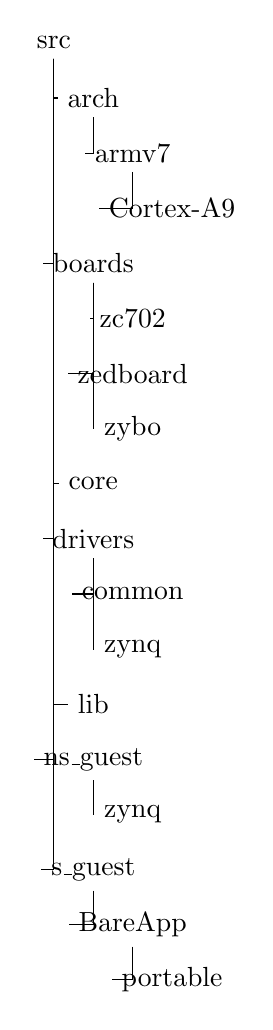
\begin{tikzpicture}[%
    grow via three points={one child at (0.5,-0.7) and %
    two children at (0.5,-0.7) and (0.5,-1.4)},%
    edge from parent path={(\tikzparentnode.south)%
    |- (\tikzchildnode.west)}]
  \node {src}
      child { node {arch}
        child {node {armv7}
        child {node {Cortex-A9}}}}
      child [missing] {}
      child [missing] {}
      child { node {boards}
        child {node {zc702}}
        child {node {zedboard}}
        child {node {zybo}}}
      child [missing] {}
      child [missing] {}
      child [missing] {}
      child { node {core}}
      child {node {drivers}
        child { node {common}}
        child {node {zynq}}}
      child [missing] {}
      child [missing] {}
      child {node {lib}}
      child {node {ns\_guest}
        child {node {zynq}}}
      child [missing] {}
      child { node {s\_guest}
        child {node {BareApp}
          child {node {portable}}}};
  \end{tikzpicture}
  \caption{Struktura direktorija izvršnog koda LTZVisora}
  \label{srcdir}
\end{figure}

Direktorij \textit{boards} sadrži skriptu za memorijsko povezivanje i kod koji je specifičan sad određenu platformu te služi
podešavanju sigurnosti uređaja (npr. TTC, UART, globalno brojilo), SLCR registra (podešavanje sigurnosti memorijskih
segmenata, sigurnosti DMA, \textit{Etherneta}, OCM...) i upravljačke programe uređaja koji se koriste (TTC i UART). Isto tako,
sadrži i inicijalizaciju GIC-a. Slijedeći direktorij, \textit{core}, sadrži jezgru LTZVisora koja je zadužena za postavljanje
početnog konteksta Nesigurnog gosta i predavanje kontrole Sigurnom gostu. \textit{drivers} direktorij sadrži upravljački
program GIC-a, a \textit{lib} funkcije za rukovanje znakovnim nizovima i pristup registrima. Slika Nesigurnog gosta se gradi
odvojeno od Sigurnog gosta i LTZVisora, koji se izgrađuju zajedno, te direktorij \textit{ns\_guest} sadrži kod za uključivanje
slike Nesigurnog gosta u sliku cjelokupnog sustava i atribute potrebne za pokretanje Nesigurnog gosta. Zadnji,
\textit{s\_guest}, direktorij sadrži kod Sigurnog gosta i tablicu prekidnih vektora Sigurnog gosta.

\chapter{Operacijski sustav Linux}
Linux je operacijski sustav otvorenog koda te je prvenstveno namijenjen stolnim računalima (spada u GPOS).
Otvorenost koda omogućila je prilagođenje Linuxa za ugradbena računala.
Rastom mogućnosti procesora za ugradbena računala, sve je veća i potražnja za operacijskim sustavom Linux za ugradbena
računala. Linux je obično tražen zbog već gotove podrške za sučelja koja su potrebna u aplikaciji koja se razvija, npr.
mrežna podrška. Važne komponente Linuxa su jezgra, datotečni podsustav i \textit{Device Tree} koji su opisani u nastavku
ovog poglavlja. Kod ugradbenih računala, datotečni podsustav i jezgra operacijskog sustava su komprimirani.
Kako bi se Linux mogao pokrenuti, nužno je imati program pokretač (npr. U-Boot) koji će pripremiti platformu za izvođenje
Linuxa. Priprema platforme sastoji se od:
\begin{itemize}
  \item{inicijalizacije memorijskog sustava i periferija}
  \item{učitavanja slike Linuxa u RAM memoriju}
  \item{predaje ulaznih argumenata Linuxu}
  \item{pripremanja serijske konzole za jezgru (ovaj korak je izborni, ako se postave odgovarajući parametri za automatsko
  pokretanje jezgre OS-a)}
  \item{predaje kontrole jezgri OS-a}
\end{itemize}
Neposredno prije nego što program pokretač skoči na početnu instrukciju jezgre Linuxa, pokretač
pripremi tri parametra koja su nužna za pokretanje Linuxa. Parametri se prenose preko registara opće namjene R0-R2, gdje
R0 mora sadržavati 0, R1 tip platforme (jedinstveni identifikator platforme) i R2 početnu adresu \textit{Device Tree} binarne
datoteke.

\section{Komponente operacijskog sustava Linux}
Kao što je već spomenuto, Linux za ugradbena računala sadrži tri glavne komponente sustava: datotečni podsustav, \textit{Device
Tree} i jezgru operacijskog sustava. Svaka od tih komponenata može biti izgrađena raznim alatima, u ovom radu je izabran
Xilinxov alat \textit{PetaLinux} koji ima mogućnost izgradnje svih komponenata odjednom. Svaka od komponenata je detaljnije
opisana u nastavku.

\subsection{\textit{Device Tree}}
\textit{Device Tree} je podatkovna struktura koja opisuje konfiguraciju hardvera kojeg će Linux koristiti. Sadrži sve potrebne
informacije o procesorima u sustavu, veličini memorije i konfiguraciji prekida i periferija. Struktura se upisuje u datoteku
ekstenzije \textit{.dts} ili \textit{.dtsi}, gdje je \textit{.dts} konačna datoteka koja može uključivati dodatne informacije
sadržane u \textit{.dtsi} datotekama \cite{xlnx}. Ako datoteke \textit{.dts} i \textit{.dtsi} sadrže informacije o istim komponentama,
u konačnici se uzima podatak iz \textit{.dts} datoteke. \textit{Device Tree} je važan jer opisuje hardver na način koji je
razumljiv Linuxu, a uz to, omogućuje Linuxu da nema fiksnu konfiguraciju hardvera \cite{plnx}. Svaki upravitelj uređajima ili modul
u \textit{Device Tree} strukturi je opisan čvorom koji sadrži sve postavke uređaja. Obzirom na vrstu upravitelja, upravitelj
može imati čvorove djece i čvor roditelja. Korjenski čvor je roditelj svim ostalim čvorovima te se sastoji od:
\begin{itemize}
  \item{čvora koji sadrži informacije o procesorima platforme}
  \item{čvor koji sadrži informacije o memoriji}
  \item{izborni čvor koji može sadržavati konfiguracijske podatke (parametre jezgre, lokaciju datotečnog podsustava...)}
  \item{čvor koji označava istoznačnice (alijase)}
  \item{čvorove koji sadrže informacije sabirnica platforme}
\end{itemize}
Sintaksa \textit{Device Tree} strukture prikazana je slikom \ref{devtree_sintax}.

\begin{figure}[H]
  \centering
  \begin{lstlisting}
    node@address{
      property_name = "property_value";
      byte_property_name = [hex1 hex2 hex3 hex4];
      child_node@address{
        reference = <&reference_node>;
      };
    };
  \end{lstlisting}
  \caption{Sintaksa \textit{Device Tree} strukture}
  \label{devtree_sintax}
\end{figure}

Binarni ekvivalent, potreban za konačnu sliku sustava, \textit{.dts} datoteke je \textit{.dtb} koja se dobije DTC (engl.
\textit{Device Tree Compiler}) alatom.

\subsection{Datotečni podsustav}
Linux je operacijski sustav koji sve upravljačke programe uređaja drži u obliku datoteka, stoga je potrebno imati datotečni
podsustav (korjenski datotečni podsustav), kako bi Linux ispravno funkcionirao. Datotečna struktura odgovara strukturi
datotečnog sustava Linuxa za stolna računala, ali uz znatno manje elemenata koji se mogu i dodatno smanjiti pomoću alata
za izgradnju datotečnog podsustava (npr. \textit{BusyBox} kojeg koristi \textit{PetaLinux}). Datotečni podsustav je obično
pohranjen u stalnu memoriju, ali postoji mogućnost i za pohranu u RAM memoriju.
Postoje različiti tipovi datotečnih podsustava, a ovo su neki od njih:
\begin{itemize}
  \item{\textit{initramfs} - datotečni podsustav koji ima mogućnost pisanja u datotečni podsustav, ali promjene nisu stalne,
  tj. gube se nakon gubitka napajanja. Izvorno mjesto ovakvog datotečnog podsustava je RAM.}
  \item{\textit{initrd} - datotečni sustav koji je prethodio \textit{initramfsu} i vrlo sličnih mogućnosti. Također se nalazi
  u RAM-u.}
  \item{\textit{jffs2} - montira se u \textit{flash} memoriju, gdje se jedna particija \textit{flasha} obavezno mora zvati
  \textit{jffs2} te se treba pobrinuti da particija ima dovoljno memorije za datotečni podsustav.}
  \item{NFS (engl. \textit{Network File System}) - datotečni sustav se montira preko mreže te ciljana platforma i sustav
  domaćin dijele isti datotečni podsustav.}
  \item{SD datotečni podsustav - sustav koji je posebno izgrađen za SD karticu.}
\end{itemize}
Novije verzije jezgre podržavaju komprimirane \textit{cpio} arhive te je iz tog razloga moguće ručno ispuniti datotečni
podsustav sa željenim sadržajem uz pomoć \textit{cpio} alata na Linuxu. Takve arhive se komprimiraju za Linux algoritmom
koji se može izabrati u izborniku alata kojim je datotečni podsustav građen.
Sadržaj datotečnog podsustava se najčešće odnosi na:
\begin{itemize}
  \item{sustavske biblioteke}
  \item{aplikacije}
  \item{alate i različite usluge (komandni sustav, \textit{web} pretraživači...)}
\end{itemize}

\subsection{Jezgra}
Izgradnje jezgre se sastoji od dva sustava:
\begin{itemize}
  \item{sustav koji je neovisan o arhitekturi za koju se jezgra gradi (raspoređivač procesa, sučelje sustavskih poziva,
  upravljački programi koji su neovisni o arhitekturi i mrežni podsustav)}
  \item{sustav koji se tiče hardvera platforme za koju se jezgra gradi (inicijalizacija platforme, uređaji vezani uz odabranu
  platformu, itd.)}
\end{itemize}
Jezgra se poziva pomoću programa pokretača koji skače na prvu instrukciju jezgre operacijskog sustava te prvo što jezgra radi je
provjera ulaznih argumenata. Ako su ulazni argumenti valjani, jezgra počinje izvršavati početni program koji se odnosi na
dekomprimiranje jezgre. Nakon što je dekomprimiranje gotovo, kreće se na inicijalizaciju sustava. Sekvenca inicijalizacije
koju izvršava jezgra:
\begin{enumerate}
  \item{Onemogućavaju se IRQ i FIQ, inicijalizira se \textit{tick} sustava, memorijski sustav, podsustavi ovisni o arhitekturi,
  uz koje se u obzir uzimaju ulazni argumenti koje je predao program pokretač}
  \item{Konfigurira se stog i raspoređivač zadataka}
  \item{Alociraju se stranice i podešavaju određena memorijska područja}
  \item{Podešavaju se prekidi, iznimke i GIC}
  \item{Brojilo korišteno kao \textit{tick} se podešava i omogućuju se prekidi te se izvodi dodatna inicijalizacija memorije i
  kalibriranje takta jezgre}
  \item{Podešava se datotečni podsustav i inicijaliziraju se procesi, izvršavaju se \textit{daemon} programi koji su zaduženi
  za stvaranje niti (engl. \textit{thread}) jezgre}
  \item{Jezgra se otključava i raspoređivač se pokreće}
  \item{Inicijaliziraju se razni uređaji i mreža}
\end{enumerate}
Važno je napomenuti da prije predaje kontrole jezgri operacijskog sustava, MMU i podatkovna \textit{cache} memorija moraju biti
onemogućeni te početno stanje jezgre mora biti u \textit{supervisor} načinu rada uz IRQ i FIQ maskirane (onemogućene). Ako
jezgra nije primila valjane ulazne argumente, izvršavanje koda jezgre se prekida uz serijski ispis odgovarajuće poruke.

\section{\textit{PetaLinux}}
\textit{PetaLinux} je skup alata koji olakšavaju izgradnju slike Linuxa. Sadržava DTC alat za prevođenje \textit{Device Tree}
strukture, za izgradnju datotečnog podsustava koristi \textit{BusyBox} te jezgru Xilinxovog Linuxa preuzima s \textit{GitHuba}.
\textit{PetaLinux} ima više verzija koje su dostupne za instalaciju, a u ovom radu se je koristio \textit{PetaLinux} 2019.1 koji
koristi verziju Linuxa 4.19. Pomoću \textit{PetaLinuxa} sučelja moguće je konfigurirati jezgru preko izbornika koji se poziva
naredbom \textit{petalinux-config -c kernel}. Iz sučelja je moguće dodati ili ukloniti razne upravljačke programe uređaja,
module ili mogućnosti jezgre. Kako \textit{PetaLinux} koristi Xilinxov Linux, izbornik sadrži mogućnosti dodavanja raznih
upravljačkih programa napisanih posebno za Xilinxove platforme, kao što je to ZedBoard. Za konfiguriranje datotečnog podsustava,
koristi se poseban izbornik koji se pokreće naredbom \textit{petalinux-config -c rootfs} koji također ima mogućnost uklanjanja
i dodavanja raznih komponenti datotečnog podsustava te ima i mogućnost dodavanja korisničkih aplikacija u datotečni  podsustav.
\textit{Device Tree} Linuxa se konfigurira pomoću datoteke koja je predviđena za dodavanje korisničkih informacija koje se tiču
hardvera. Opće postavke cjelokupne slike sustava mogu se postaviti pomoću općenitog izbornika koji se poziva naredbom
\textit{petalinux-config}. Početni sadržaj ovog izbornika je prikazan slikom \ref{peta_menu}.
\begin{figure}[H]
  \centering
	\includegraphics[width=300pt]{peta_menu.png}%
	\caption{Izbornik \textit{petalinux-config} naredbe}
	\label{peta_menu}%
\end{figure}
Pomoću prikazanog izbornika
moguće je odabrati razne općenite postavke slika koje se generiraju naredbom \textit{petalinux-build}. Najvažnije postavke
se odnose na početnu adresu na kojoj će se nalaziti slika jezgre u memoriji i cjelokupna memorija koja je dostupna Linuxu.
Uz to, ovim izbornikom je moguće odabrati željenu vrstu datotečnog podsustava (gdje su ponuđene vrste koje su navedene u
prethodnim poglavljima). Navedenim izbornikom se mogu upravljati i nekim postavkama \textit{Device Tree} strukture. Velik dio
postavki se odnosi na upute U-Bootu kako pronaći i pokrenuti jezgru operacijskog sustava. Vrlo korisni dio za početnike je
izbor \textit{Help} koji daje detaljniji opis ponuđenih komponenti te daje upute nesigurnom korisniku može li ukloniti
određene komponente iz Linuxa. Još jedna korisna postavka koju nudi \textit{PetaLinux} je mogućnost stavljanja eksternog
izvora Linuxovog koda što je posebno važno kod aplikacija koje zahtijevaju izmjenu izvornog koda jezgre.\\
Uz instalacijski paket \textit{PetaLinuxa}, preuzmu se i razni predlošci koji olakšavaju stvaranje inicijalnog
\textit{PetaLinux} projekta za odgovarajuću platformu s inicijalnim postavkama koje su valjane za odabranu platformu. Nakon
izgradnje sustava, slika jezgre Linuxa za Zynq-7000 platforme je naziva \textit{zImage} te je slika komprimirana. Ako se
za datotečni podsustav odabere \textit{initramfs}, komprimirana slika datotečnog podsustava je automatski sadržana u
\textit{zImage} slici. Binarni oblik \textit{Device Tree} strukture je generiran u datoteku naziva \textit{system.dtb}.

\section{Prilagođenje Linuxa kao Nesigurnog gosta LTZVisora}
Preporuka ARM-a je da složeniji operacijski sustavi budu namijenjeni Nesigurnom svijetu, jer je kod sustava s većom
količinom koda veća vjerojatnost pronalaženja prolaza do probijanja sigurnosti. Zbog toga razloga, autori LTZVisora također
preporučuju implementaciju GPOS-a kao Nesigurnog gosta. Prilagođenje kompleksnog sustava kao što je to Linux za Nesigurni
svijet \textit{TrustZone} platforme je posao koji zahtjeva vrlo dobro poznavanje arhitekture jezgre operacijskog sustava, kao
i detaljno poznavanje platforme za koju se Linux prilagođava. Pristup prilagođenju može biti sljedeći: ako se Linux priprema
za Nesigurni svijet, ključno je omogućiti konfiguriranje jezgre koje zahtjeva pristup sigurnoj memoriji, odnosno registrima
kojima može pristupiti samo Sigurni svijet. Ovakav pristup, odmah u početku, uklanja potrebu za detaljnim poznavanjem
dijela jezgre operacijskog sustava koji je neovisan o arhitekturi platforme što znatno smanjuje vrijeme prilagodbe jezgre
Nesigurnom svijetu. Uz takav pristup, jasno je i da se \textit{Device Tree} mora promijeniti. Prilagođenje Linuxa se sastoji
i od pripreme LTZVisora za Linux te su postupci prilagodbe dani u nastavku.

\subsection{Stvaranje cjelokupne slike Linuxa}
Arhitektura LTZVisora zahtjeva jednu izvršnu datoteku Nesigurnog gosta, dok se Linux sastoji od više slika sustava (datotečnog
podsustava, \textit{Device Tree} strukture i jezgre). Uz to, Linux zahtjeva i program pokretač koji će pripremiti jezgru za
početak izvršavanja. Jasno je da je potrebno sve slike sustava Linux i program pokretač povezati u jednu izvršnu datoteku
koju će LTZVisor kasnije učitati u RAM. Jedan od intuitivnih načina na koji to postići je pomoću skripte za memorijsko
povezivanje u kojoj su naznačene adrese za svaku komponentu operacijskog sustava Linux. U ovom radu se je iskoristila mogućnost
koju nudi \textit{PetaLinux}, a tiče se vrste datotečnog podsustava. Kao vrsta datotečnog podsustava odabrao se
\textit{initramfs} zbog mogućnosti da je takav datotečni podsustav odmah uključen u sliku jezgre Linuxa što doprinosi smanjenju
otiska cjelokupne slike Linuxa. Kada bi se koristio drugi datotečni podsustav, u skriptu za memorijsko povezivanje bilo bi
potrebno dodati poseban adresni prostor koji sadrži datotečni podsustav koji najvjerojatnije ne bi bio u potpunosti popunjen.
Sve što je potrebno u skripti za memorijsko povezivanje je adresa na kojoj se sprema \textit{Device Tree}, adresa minimalnog
koda koji predaje parametre jezgri Linuxa i adresu na kojoj se nalazi jezgra. Adrese na kojima su smještene komponente Linuxa
su prikazane tablicom \ref{adr_space}.
\begin{table}[H]
  \centering
  \begin{tabular}{ | p{3cm} | p{6cm} |}
    \hline
    \textbf{Adresa} & \textbf{Slika}\\
    \hline
    0x2000000 & \textit{Device Tree}\\
    \hline
    0x2007000 & Program pokretač\\
    \hline
    0x2008000 & Jezgra i datotečni podsustav  Linuxa\\
    \hline
  \end{tabular}
  \caption{Adresni prostor komponenata Linuxa}
  \label{adr_space}
\end{table}
Program pokretač se sastoji od jedne funkcije koja predaje potrebne parametre jezgri Linuxa i skače na početnu adresu jezgre.
Početna funkcija jezgre se može identificirati pomoću alata \textit{arm-none-eabi-objdump} koja ima mogućnost iz binarne
datoteke ispisati niz asemblerskih instrukcija ili simbola koje sadrži izvršna datoteka. Najjednostavnije je iskoristiti
navedeni alat za ispis tablice simbola sadržanih u izvršnoj datoteci. Ispisom simbola vidi se da se početna točka jezgre
Linuxa naziva \textit{\_binary\_images\_linux\_zImage\_start} koja se može iskoristiti kao funkcija s tri ulazna argumenta.
Ulazni argumenti su redom: R0, R1 i R2, gdje R0 sadrži 0, R1 jedinstveni identifikator ZedBoarda koji je 3378 i početna adresa
\textit{Device Tree} strukture koja je definirana u skripti za memorijsko povezivanje (0x2000000). Prije nego se sve slike
povežu u konačnu sliku, potrebno je konvertirati sliku jezgre i \textit{Device Tree} u binarne datoteke pomoću alata
\textit{arm-none-eabi-objcpy}. Nakon toga, slike se mogu povezati u jednu koja se može iskoristiti za LTZVisor.

\subsection{Izmjene u jezgri operacijskog sustava}
\subsection{Izmjene u LTZVisoru}

\chapter{Operacijski sustav za rad u stvarnom vremenu (RTOS)}
\section{FreeRTOS}
\subsection{Programska podrška za Zynq-7000}
\subsection{Prilagodba FreeRTOS-a kao Sigurnog gosta LTZVisora}

\chapter{LTZVisor za višejezgrene procesore}
\section{Prilagođenja LTZVisora za AMP}
\subsection{Arhitektura AMP LTZVisora}
\subsection{Nadgledni način rada CPU0}
\subsection{Nadgledni način rada CPU1}
\section{Prilagođenja LTZVisora za SMP}
\subsection{Arhitektura SMP LTZVisora}
\subsection{Promjene u nadglednom načinu rada procesora}
\subsection{Promjene u Nesigurnom \textit{bare-metal} gostu}
\subsection{Promjene u SMP Linux Nesigurnom gostu}

\chapter{Testiranje LTZVisora za višejezgrene procesore}

\chapter{Zaključak}
Zaključak.

\bibliography{literatura}
\bibliographystyle{fer}

\begin{sazetak}
Sažetak na hrvatskom jeziku.

\kljucnerijeci{Ključne riječi, odvojene zarezima.}
\end{sazetak}

% TODO: Navedite naslov na engleskom jeziku.
\engtitle{Title}
\begin{abstract}
Abstract.

\keywords{Keywords.}
\end{abstract}

\end{document}
